% siminos/blog/Mathematica.tex
% $Author: predrag $ $Date: 2016-04-13 20:36:35 -0400 (Wed, 13 Apr 2016) $
%    this is master file: siminos/cgang/2modes.tex
%    \section{{\twoMode} daily blog}
%    \label{chap:2modes}


\subsection{Blogging simulations progress}
\label{s:MathematicaBlog}

\begin{description}
\item[2012-06-11 Predrag]
started a new blog, for Chaos Gang {\twoMode} simulations.

\texttt{siminos/blog/Mathematica.tex}

\item[2012-04-25 Evangelos]
Wrote an interactive Mathematica program, with sliders for parameters:

\texttt{siminos/cgang/Evangelos/dangelmayr\_so2\_int.nb}

\item[2012-04-25 Evangelos]
Dangelmayr system with Predrag's modification
becomes very interesting. It's very easy to find chaotic behavior and in many
cases it seems that asymptotic dynamics are $3$-dimensional.
After spending some time playing with parameters, I've found some
for which it seems we have chaos (at least we can see some stretching
and folding) while a $2$-dimensional description might be possible
(a simple $2$-d branched manifold).
The parameters are
\bea
 \mu_1 &=& -0.337,\, \mu_2 = 0.27,\, c_1 = 1,\, c_2 = -1,\, a_1 = -1.5,\,
\continue
 a_2 &=& -6.19,\, b_1 = 1.583,\,  b_2 = -0.115,\, e_2 = 1.211
 \,.
\label{pars2012-04-25}
\eea
I would suggest playing with \texttt{siminos/cgang/Evangelos/dangelmayr\_so2\_int.nb}
to locate \emph{nearby} parameters which you think will give more interesting
results or just explore the system with the parameters given here.

%%%%%%%%%%%%%%%%%%%%%%%%%%%%%%%%%%%%%%%%%%%%%%%%%%%%%%%%%%%%%%%%%%%%%%%%%%%%%%%%%%%%
 \begin{figure}
%% ES created with siminos/cgang/Evangelos/dangelmayr_so2_plot.nb
\centering
 (a) 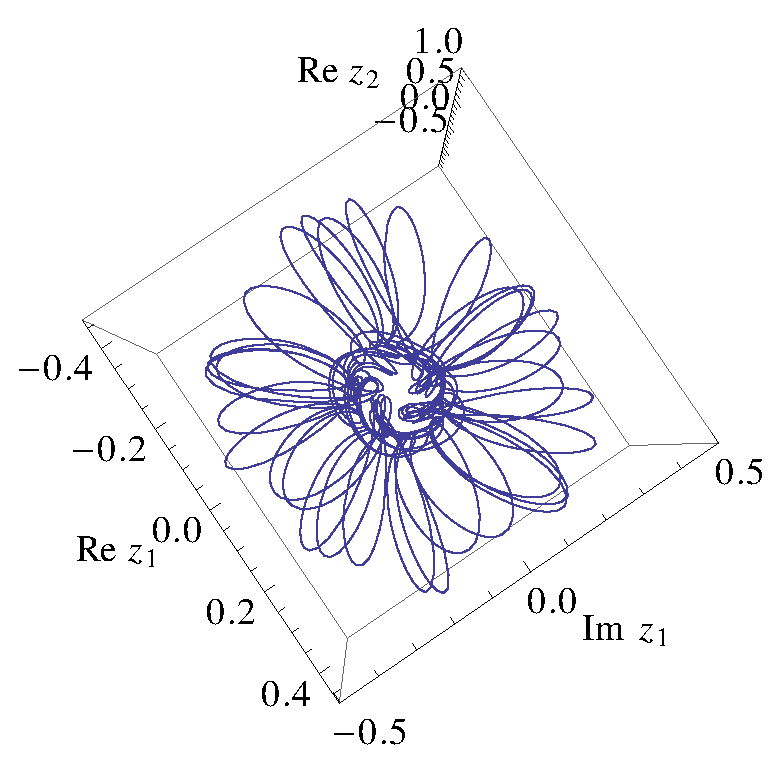
\includegraphics[width=0.35\textwidth]{dangelmayrZ}~
 (b) 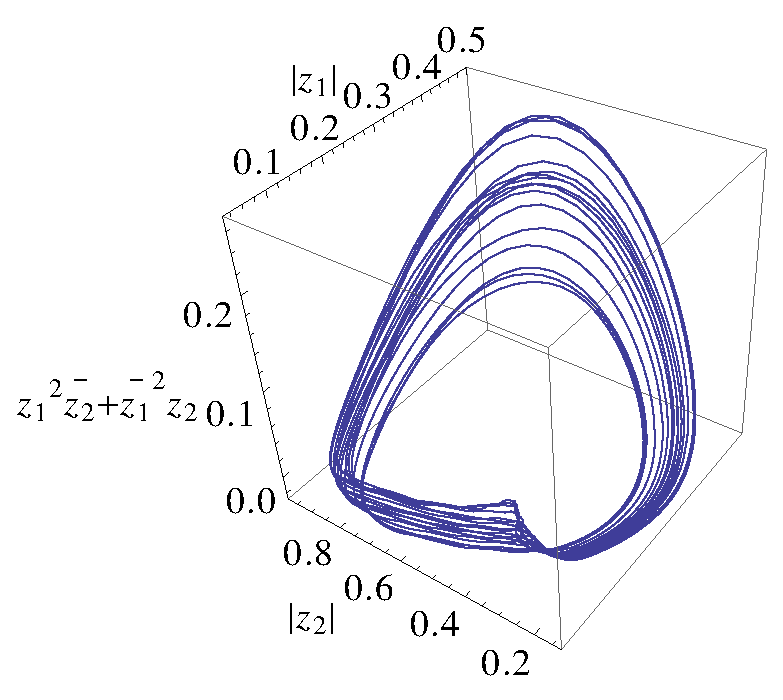
\includegraphics[width=0.35\textwidth]{dangelmayrAGH}~
\caption{Projections of Dangelmayr system \refeq{eq:DangSO2}
``attractor'' for parameters \refeq{pars2012-04-25} in
(a) equivariant \statesp\ coordinates
    $\{x_1, y_1 ,x_2, y_2\}$
    % $\Re z_1,\,\Im z_1,\,\Re z_2$.
(b) invariant coordinates
    $\{\sqrt{u}, \sqrt{v}, w\}$
% used by Armbruster \etal\rf{AGHO288}
% $|z_1|,\, |z_2|,\, z_1^2 \bar{z}_2 + \bar{z}_1^2 z_2$.
}
 \label{fig:dangelmayrChaos}
\end{figure}
%%%%%%%%%%%%%%%%%%%%%%%%%%%%%%%%%%%%%%%%%%%%%%%%%%%%%%%%%%%%%%%%%%%%%%%%%%%%%%%%%%%%%

\item[2012-04-21 Evangelos]
The Dangelmayr system\rf{Dang86} written in complex coordinates $z_1,z_2$
is given in \refeq{eq:DangSO2} I have replaced symmetry breaking term $e$
here and in \refeq{eq:AGpolar} with $e_2$ since in this constant is
naturally paired with $\mu_2$. See also Armbruster, Guckenheimer and
Holmes\rf{AGHO288} flow with $\On{2}$ symmetry, here \refeq{eq:AGH}. In
\texttt{siminos/cgang/Evangelos/dangelmayr\_so2\_int.nb} I integrate
\refeq{eq:DangSO2} rather than the polar form \refeq{eq:AGpolar}, as the
former has no dangerous denominators.

\item[2012-04-25 Evangelos] Yet another snapshot of {\twoMode}
system with Predrag's modification, for different parameters. This looks
like an attractor made of two pieces, so it might be complicated enough
to demonstrate slicing. However I have yet no insight on whether there
are really two distinct topological mechanisms hidden here and what
controls them. Once relative equilibria are located, we should add them
here. The parameters are
\bea
 \mu_1 &=& -0.337,\, \mu_2 = 0.27,\, c_1 = 1,\, c_2 = 1, a_1 = -1.4,
\continue
 a_2 &=& -6,\, b_1 = 1.6,\,  b_2 = -0.1,\, e_2 = 1.217, e_1 = 0
 \,.
\label{pars2012-04-25}
\eea
\item[2012-08-10 Predrag] Not a good choice - please follow Chossat\rf{Choss01}
and always use $c_1c_2<0$, as suggested by {\bf [2012-08-06 Knobloch]}.

%%%%%%%%%%%%%%%%%%%%%%%%%%%%%%%%%%%%%%%%%%%%%%%%%%%%%%%%%%%%%%%%%%%%
 \begin{figure}[h]
%% ES created with siminos/cgang/Evangelos/dangelmayr_so2_plot.nb
\centering
 (a) 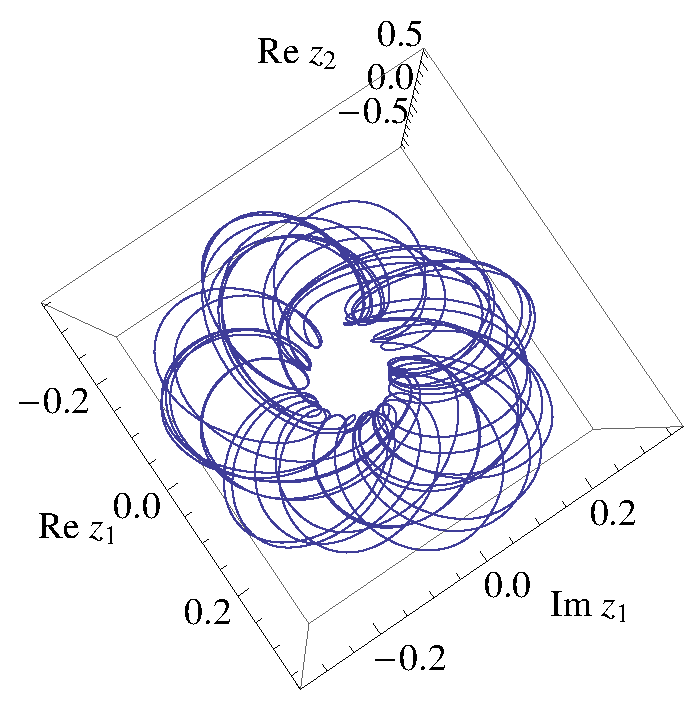
\includegraphics[width=0.35\textwidth]{dangelmayrZ2}~
 (b) 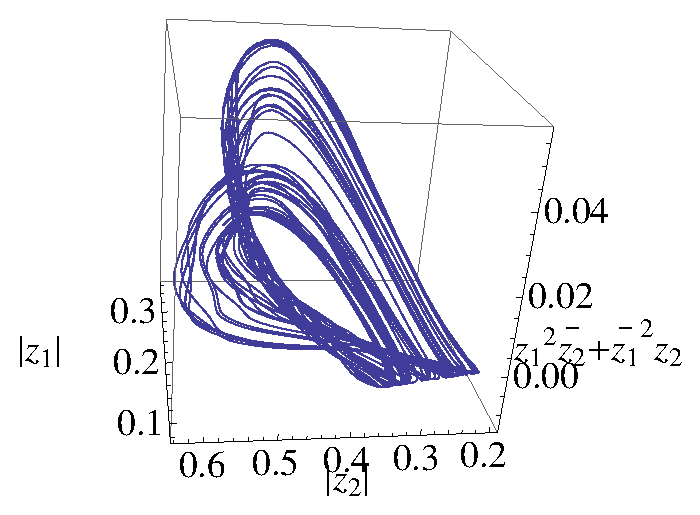
\includegraphics[width=0.35\textwidth]{dangelmayrAGH2}~
\caption{Projections of Dangelmayr system \refeq{eq:DangSO2}
``attractor'' for (not a good choice) parameters \refeq{pars2012-04-25}, in
(a) original state space variables $\Re z_1,\,\Im z_1,\,\Re z_2$.
(b) invariant coordinates used by
Armbruster \etal\rf{AGHO288}
$|z_1|,\, |z_2|,\, z_1^2 \bar{z}_2 + \bar{z}_1^2 z_2$.
}
 \label{fig:dangelmayrChaos2}
\end{figure}
%%%%%%%%%%%%%%%%%%%%%%%%%%%%%%%%%%%%%%%%%%%%%%%%%%%%%%%%%%%%%%%%%

\item[2012-04-27 Predrag] \refFig{fig:dangelmayrChaos2}\,(b) is one of 4
projections from the 4\dmn\ invariant polynomials $\{u,v,w,q\}$ dynamics
on any three of them. I would prefer that all such projections are linear
in coordinates (otherwise small $z_i$ really get scrunched), so please
plot $\{|u|^{1/2},|v|^{1/2},w/u |v|^{1/2} ,q/u |v|^{1/2} \}
= \{r_1,r_2, \cos\psi, \sin\psi \}$, or similar...

\item[2012-04-25 Bryce] In the spirit of ``experimenting'' I flipped the
sign of b2 from -0.1 to .01 and got the following plots. Not sure what to
make of them though... My brain needs some fuel and my eyes are starting
to strain so I'm throwing the towel in for now in favor of some food.

\begin{figure}[H]
\centering
 (a) \includegraphics[width=0.35\textwidth]{pkTraj2}
 (b) \includegraphics[width=0.35\textwidth]{pkTraj2Reduced}
\caption{Projection of Dangelmayr system \refeq{2mode4Da}
``attractor'' for parameters \refeq{pars2012-04-25a}.
(a) Projection onto original state space:
$(|z_1|,|z_2|,z_1^2\overline{z_2}+\overline{z_1}^2 z_2)$. (b) Symmetry
reduced trajectory using the following template for the slice $(0.220299,
0.784274, -1.03596, 2.46552)$.
}
\label{fig:pkfig2}
\end{figure}

\bea
 \mu_1 &=& -0.337,\, \mu_2 = 0.27,\, c_1 = 1,\, c_2 = 1,\, a_1 = -1.4,
\continue
 a_2 &=& -6,\, b_1 = 1.6,\,  b_2 = 0.1,\, e_2 = 1.217
 \,.
\label{pars2012-04-25a}
\eea
\item[2012-08-10 Predrag] Not a good choice - please follow Chossat\rf{Choss01}
and always use $c_1c_2<0$, as suggested by {\bf [2012-08-06 Knobloch]}.

\item[2012-04-27 Predrag] Experimenting is great, but please read what I
have written, and either show me that I am wrong, or experiment
accordingly. Here are clips of above unread text:

(clip 1) As we want hyperbolicity, pick $\mu_j$ of opposite signs. In
order to avoid the \cLe\ near visits to the invariant subspace (there it
was the $z$ axis, here it is the $m=2$ subspace) pick contraction within
the subspace, $\mu_2 < 0$, but make it overall repelling by making sure
that $\mu_1 > -\mu_2 > 0$. No parameters that you have reported chaos for
so far satisfy that.

(clip 2) \refFig{fig:pkfig1}\,(b) is one of 4
projections from the 4\dmn\ invariant polynomials $\{u,v,w,q\}$ dynamics
on any three of them. I would prefer that all such projections are linear
in coordinates (otherwise small $z_i$ really get scrunched), so please
plot $\{|u|^{1/2},|v|^{1/2},w/u |v|^{1/2} ,q/u |v|^{1/2} \}
= \{r_1,r_2, \cos\psi, \sin\psi \}$, or similar...

\item[2012-04-27 Keith to Predrag] I know what your suggestions are for
$\mu_1$ and $\mu_2$, but I found the origin never to have much an effect
on any of the dynamics, so I went and tried some other stuff.  What I
found when I symmetry reduced was what appears to be two R\"ossler like
trajectories floating around two equilibrium and a single trajectory
visiting both: \reffig{fig:2moderedmultieq}.  I post processed this
trajectory rather than running the dynamics in the slice, and the slice
was: $[1, 0, 0, 0]$ which is rather unoriginal, but it provided the
easiest condition for rotating the frame at the time, because once I
found these parameters, I thought there might be some interesting events
to these.  The problem, of course with this slice is that the invariant
space $r_1 = 0$ remains a circle.
    The parameters are (not a good choice) \refeq{pars2012-04-25}.

\item[2012-04-28 Predrag] Wow, this is beautiful. Victoria Secret's Pink
line. The three dots are the \eqv\ and two rather similar \reqva, both
spiral-out unstable? Is the $m=2$ subspace ($r_1 = 0,\, r_2 > 0$) \reqv\
where Daniel says it is? Stable, unstable? Whatever `slice' means (there
are rumors of a good paper defining it, but's not on arXiv yet), it is
not $[1, 0, 0, 0]$. No habla esta idioma. You mean template $\slicep =
[1, 0, 0, 0]$ or group tangent $\sliceTan{} = [1, 0, 0, 0]$? Presumably
$\sliceTan{} = [1, 0, 0, 0]$. Not obvious to me that \reqv\ in $m=2$
remain a circle, but there surely is one (attractive?) that seems to give
shape to the hot pants. You seem to have set $x_2=0$ (that is $m=2$
coordinate?)

Time to go to bed...

\item[2012-04-28 Keith] I reposted the images for parameters I gave last
night.  I changed the colors of all the (\reqva) to be able
to talk about them.  I have given you a point in terms of $[x_1, x_2,
y_1, y_2]$ where $x_1$ and $x_2$ are the first mode and $y_1$ and $y_2$
are the 2nd mode.
\begin{itemize}
    \item[Black] $[0,0,0,0]$ with eigenvalues: $(1+2i,1-2i,2,2)$
    \item[Green] $[0,0,-0.14462,-0.650791]$ or in $(r_1, r_2, \psi)$
    coordinates $[0, 0.6667, ?]$ the $\psi$ doesn't matter; with eigenvalues:
    $(-6.44444,6.88889,-1 \pm 1.73205\ii)$
    \item[Blue] $[0.358405,0,0.00733041,-0.526708]$
    with eigenvalues: $(-3.57283 \pm 10.3177i,2.03058 \pm 7.89832\ii)$
    \item[Cyan] $[0.39517,0,0.00742352,0.475084]$
    with eigenvalues:  $(-3.05375 \pm 10.5197i,1.48008 \pm 9.80073i)$
\end{itemize}

\begin{figure}[H]
\centering
 (a) \includegraphics[width=0.35\textwidth]{kc2modesideview.png}
 (b) \includegraphics[width=0.35\textwidth]{kc2modedownthebarrel.png}
 (c) \includegraphics[width=0.35\textwidth]{kc2modeturnedview.png}
 (d) \includegraphics[width=0.35\textwidth]{kc2modelastview.png}
\caption{
(a) Symmetry reduced Hot Pants trajectory, side perspective.
(b) Symmetry reduced along the $r_1$ axis.
(c) Another perspective around one of the \reqv. (d)
Perspective around the other \reqv.
Finding the best angles to do this was difficult, so if you want an
interactive version, I can post it. The parameters are given as:
    $\mu_1 = \, a_2 = $
}
\label{fig:2moderedmultieq}
\end{figure}

\bea
 \mu_1 &=& 2.0 ,\, \mu_2 = 1.0,\, a_1 = -7.5,
\continue
 a_2 &=& -2,\, b_1 = -4,\, b_2 = -2.25,\, c_1 = 10,\, c_2 = -35,\, e_2 = 2
 \,.
\label{pars2012-04-28}
\eea
\item[2012-08-10 Predrag] Not a good choice we use $c_j = \pm 1$.


\item[2012-04-28 Predrag] \refFig{fig:2moderedmultieq} attractor (what is it ?) is sexy and she
knows it.

According to {\bf [2012-04-27 Daniel]},
the $[0,0,0,0]$ eigenvalues are $\lambda_1 = \mu_1$ with multiplicity 2 and
             $\lambda_3 = \mu_2 \pm i e_2$. The eigenvectors for
             $\lambda_1$ are $(1,0,0,0)$ and $(0,1,0,0)$ in the
             $(x_1,x_2,y_1,y_2)$ basis.
             The eigenvectors for
             $\lambda_2$ are $(0,0,1,0)$ and $(0,0,0,1)$
For your parameter values
             $\lambda_1 = \lambda_2= 2$,
             $\lambda_{3,4} = 1 \pm  2\,\ii$, it checks.

{\bf [Green]} $m=2$ invariant subspace: which of the eigenvalues' eigenvectors
    point into the $m=2$ world? Presumably $(-6.44444,6.88889)$.
    According to my suggestions for invariant subspaces, we would like
    repelling directions to win, which I think means $\lambda_1+\lambda_2
    >0$. If so, $(-6.44444,6.88889,-1 \pm 1.73205\ii)$ barely wins.
    However, if $\sum \lambda_j >0$ is the correct criterion, than contraction
    wins, which might be the reason that you seem to be coming closer and
    closer to the green \rpo.

{\bf [Blue]} and {\bf [Cyan]} \eqva\ might look cooler if the real part
of the expanding eigenvalue was a bit closer to zero - but maybe it does
not matter, as they rotate very fast (large imaginary parts). It could be
that because the contraction $-3.57283$ wins over the expansion $2.03058$
your attractor look like the heteroclinic connections of Armbruster,
Guckenheimer and Holmes,\rf{AGHO288}.

It's your {\bf [Green]} unreduced \rpo\ that blows wind into these Hot
Pants - green should be a point, and than these surfaces will shrink into
heteroclinic trajectories in \reducedsp?

And I really would be much happier if you used the full \statesp\ \eqva\
as templates, as is the current religion, even though it might mean
losing your Pants.  You really want a \slice\ which also reduces the
rotations within the $m_1=0$ invariant subspace.

\item[2012-04-28 Predrag] The Hot Pants do not look chaotic.  You'll have
to wade deeper. If \reffig{fig:2moderedmultieq} is in a slice hyperplane,
how wild is the full \statesp\ attractor?

\item[2012-04-28 Evangelos to Keith] \reffig{fig:2moderedmultieq} looks like a transient
to a stable limit cycle to me. You do plot $t=0$ to $t=t_{max}$, right? Why don't
you post a figure going from $t=t_{max}/2$ to $t_{max}$?

\item[2012-04-28 Keith to Evangelos]  Yes I actually did that this
morning, it turns out that it is a limit cycle.  So sadly this is not a
good situation to use.

\item[2012-04-28 Evangelos to Chaos Gang] Predrag and I do not like a
\reducedsp\ in which a \reqv\ (such as the green orbit in
\reffig{fig:2moderedmultieq}) does not appear as a single point. I read
the explanation in [2012-04-28 Keith to Predrag] but are we sure we don't
want to symmetry reduce within invariant subspaces? {\bf [2012-04-28
Keith]} I never intended to use this as the invariant subspace, I just
needed something to cut through the symmetries to see what was happening
instead of the full space.  I regret not having used the insights that I
gained in the chaos course.  [2012-04-29 Keith] I did not write that last
sentence, but find it rather amusing.

\item[2012-04-29 Predrag to Daniel]
% Thanks for fixing the pesky factor of 2 as well.
To summarize: \twoMode\ \reqva\ are the zeros of:
\bea
\tilde{f}(\tilde{u},\tilde{v}) &=&
  \tilde{u}\,A_1 - \tilde{v}\,A_2 = 0
\,,\qquad\qquad\qquad  deg(\tilde{f}) = 2
\continue
\tilde{g}(\tilde{u},\tilde{v}) &=&
 \left(A_1^2
 - c_1\,\tilde{v}\right)
 \left(\tilde{u}+2\,\tilde{v}\right)^2
 +e_2^2\,\tilde{v}^2 = 0
\,,\qquad  deg(\tilde{g}) = 4
\continue
 && \mbox{where }
A_1 = \mu_1+\tilde{a_1}\,\tilde{u}+\tilde{b_1}\,\tilde{v}
\,,\quad
A_2 = \mu_2+\tilde{a_2}\,\tilde{u}+\tilde{b_2}\,\tilde{v}
\,,
\nnu %\label{PKinvEqs5a}
\eea
in the positive $\tilde{u},\tilde{v} > 0$ quadrant (see
\refeq{PKinvEqs5a} for details). $g(u,v)$ and especially $f(u,v)$ look
pretty simple, so I'm thinking one can simply color-code their signs
(zeros are then 'nodal lines'). The \reqva\ are the intersections of two
sets of curves - might be a quick way to develop an intuition about roles
of various parameters, especially if you code it as something interactive
where parameters are sliders.

\item[2012-04-30 Predrag to C Gang] Evangelos
\texttt{Evangelos/dangelmayr\_so2\_int.nb} is a really cute toy - try it!

\item[2012-04-30 Predrag to Evangelos] I suggest using the 8 (or 7)
parameters of the rescaled \refeq{PKinvEqs5a} (hope I introduced no
further errors), and showing the value of a parameter under its slider
(at least, I cannot see it). There will be a bunch of constraints on the
parameters, Daniel and I will list them in as we find them.

\item[2012-04-30 Evangelos to Predrag] You can see the value of a parameter by
clicking on the cross next to the slidebar. I'll see if I can make it appear
permanently. I switched to unscaled variables while debugging the code but
I'm thinking not to switch back. The reason is that $c_1$ and $c_2$ in
Dangelmayr's paper can only take the values $\pm1$ and I follow this in
\texttt{dangelmayr\_so2\_int.nb}, so the gain in search space reduction is
not huge compared to the potential errors if I use 2 sets of parameters.
Also it keeps the code more readable. If we relax
restrictions on $c_1$, $c_2$, I will certainly switch to scaled variables.

\item[2012-05-02 Evangelos to Predrag] Now parameter values appear  bellow
sliders by default (thanks to local Mathematica expert Achilleas Lazarides).

\item[2012-04-30 Evangelos] In \texttt{siminos/cgang/Evangelos/dangelmayr\_so2\_int.nb}
I plot nullclines of \refeq{PKinvEqs5} to help with counting the number of
zeros. You can use some slidebars to vary parameters and experiment. You can
also experiment with phase-space plots of a typical trajectory and any relative
equilibria found numerically.

\item[2012-04-30 Evangelos] In \texttt{dangelmayr\_so2\_int.nb}, apart from
the nullclines, I plot the zero contour of $w^2+q^2-4u^2v$ to check whether
the syzygy is satisfied. It appears that the latter coincides with the $g(u,v)=0$
contour. Where does this come from? In deriving $f(u,v)=g(u,v)=0$ we did not
use the syzygy (at least not when I rederived it), so I thought it would impose
a further constraint satisfied exactly at the intersection of $f(u,v)=0$,
$g(u,v)=0$ for valid solutions. Why does it instead coincide with $g(u,v)$?

\item[2012-04-30 Evangelos to Predrag] I've tried your $\mu_1>-\mu_2>0$
suggestion but I cannot detect an interesting case. On the other hand with
$\mu_2>-\mu_1>0$ I find chaos but no relative equilibria. We need to get more
insight into stability of relative equilibria.


\item[2012-05-04 Sarah]
\HREF{http://www.snippyhaines.net/demos/cdf_index.htm}{Here's a first
stab} at an interactive R\"ossler web page.  It works on IE, but only
somewhat on Firefox.

\item[2012-05-06  Predrag to Sarah]
You might want to try to turn \texttt{Evangelos/dangelmayr\_so2\_int.nb}
into a {\twoMode} Wolfram CDF demonstration - it has sliders for various
parameters, and it should just work off the bat. We still have to settle
on a good example of chaos that requires two templates.

\item[2012-07-30 Evangelos] In \texttt{Evangelos/dangelmayr\_so2\_int.nb}
I now color-code the $(u-v)$-plane according to the sign of
\refeq{2ModeStabTraceES} when plotting the zero-contours of $f(u,v)$ and
$g(u,v)$ to help in detecting a parameter region with two hyperbolic
relative equilibria.

\item[2012-07-30 Evangelos] I've allowed for $e_1 \neq 0$ in
\texttt{Evangelos/dangelmayr\_so2\_int.nb}, in order to allow for a
second ``frequency'' in the system, maybe generating richer dynamics.
Have not played with it yet. Expressions used to locate (relative)
equilibria need to be modified accordingly.

\item[2012-08-06 Predrag]
Attractor for
\bea
 \mu_1 &=& -0.38,\, \mu_2 = 0.38,\, c_1 = -1,\, c_2 = 1,\, a_1 = -1.31,\,
\continue
 a_2 &=& -2.6,\, b_1 = 1.504,\,  b_2 = 0.22,\, e_2 = 1.61
 \,.
\label{pars2012-08-06}
\eea
looks pretty chaotic. Can you check what \eqva\ it has, and their
stabilities?

\item[2012-08-07 Daniel] Here's a breakdown of the stability of the
\eqva\ that we know analytically for the parameter values suggested by
Predrag. I first converted these 4\dmn\ Cartesian coordinates and then
calculated their stability in that representation.

The origin is hyperbolic with eigenvalues $\lambda_{1,2} = \mu_2 \pm i
e_2 = 0.38 \pm i 1.61$ and $\lambda_{3,4} = \mu_1 = -0.38$.

I believe \reqv\ at $\left(r_1,r_2,\psi\right) =\left(0,\sqrt{-\mu_2 /
b_2}, sin^{-1}\left(\frac{e_2}{2 c_1}
\sqrt{\frac{-b_2}{\mu_2}}\right)\right)$ does not exist (if
$(x_1,x_2,y_1,y_2) \in \mathbb{R}$) for these parameter values as per my
discussion in the blog on 2012-04-27.

\Reqv\ \refeq{invroot2a} is hyperbolic with eigenvalues $\lambda_{1,2} = 0.0923
\pm i 2.0682$, $\lambda_3 = -0.7630$, and $\lambda_4 = 0.2851$. This is
kind of confusing... shouldn't there be one eigenvector in the symmetry
direction with eigenvalue $0$? Maybe I'm messing up converting from
$(u,v,w,q)$ to $(x_1,x_2,y_1,y_2)$? I get $(0.1809,0.4102,0,-0.1437)
\rightarrow (0.3007,0.3007,0.6405,0)$ where I have converted between the
two basis by first converting the invariant coordinates to polar
coordinates and then converting the polar coordinates to Cartesian
coordinates.

Not sure how to use Evangelos's Mathematica code to find the other \eqva .

\item[2012-08-10 Evangelos] There is a function reqbPar which finds
relative equilibria as a function of the parameters. It solves
\refeq{PKinvEqs5} numerically, so I am not sure whether it finds all
roots.

\item[2012-08-08 Daniel] Tried finding further equilibria by finding
numerical solutions to $[\dot{u},\dot{v},\dot{w},\dot{q}] = 0$ for the
parameters suggested by Predrag. Only find Bryce's equilibrium and the
origin. There are a couple of roots ($[-0.3492,0.0351,-0.0909,0.0940]$
and $[0.0000,-1.7273,-0.0000,-0.0000]$) that do not satisfy the
constraints that $u,v \geq 0$. There are four further roots where
$[u,v,w,q]$ are complex. For more details see,
\texttt{/cgang/Daniel/Matlab/PKRoots.m}

Then I went through all the roots that I found and checked to see if they
satisfy the syzygy. The origin and all the unphysical (both real and
complex) solutions do, but Bryce's solution doesn't. Evaluating the
syzygy gives me $-0.033$. What does that mean? My gut feeling is that
this equilibrium is accessible to the system if you start it at some
generic point in $(u,v,w,q)$-space but not if you start in
$(x_1,x_2,y_1,y_2)$-space.

\item[2012-08-08 Predrag]
The syzygy \refeq{eq:syzPK} is sacred, so there is an error in Bryce's
solution.

\item[2012-08-09 Daniel to Predrag] You are more learned than I but I
don't know... If I search for the \eqva\ of \refeq{PKinvEqs1} with the
parameters \refeq{pars2012-08-06} numerically, I find a root that
corresponds to the value of Bryce's analytical expression
\refeq{invroot2} evaluated for \refeq{pars2012-08-06}. This is without
telling the computer anything about Bryce's solution. Plugging in his
analytical solution into \refeq{PKinvEqs1} symbolically also satisfies
the conditions for an equilibrium, except it doesn't satisfy the syzygy.

\item[2012-08-10 Predrag] See \refeq{BryceNoSolu}: it is no solution.

\item[2012-08-08 Daniel] I know we don't like Lyapunov exponents, but
since I already had the code written up from a long time ago and all I
had to do was give it the equations of motion and the Jacobian, I
calculated them out anyway for Predrag's parameters
\refeq{pars2012-08-06}. The code uses the method proposed by Eckmann and
Ruelle\rf{eckerg}. Anyway, the Lyapunov spectrum is $\approx
(0.1,0,0,-0.2)$ with a Kaplan-Yorke dimension of $D_{KY} \approx 3.4$.

\item[2012-08-08 Predrag]
Not that prejudiced (read \texttt{siminos/Lyapunov} blog). That looks
right, this has a chance of being a strange attractor - two dimensions
are trivial (symmetry has not been reduced), the remaining $1.4$ feels
too big.

But why don't you do the easy thing that you already have code for - take
a point on the strange attractor as a template, and run in the \slice\
hyperplane until the angle \refeq{chartBordAng} gets small? It's easier
than thinking, and we just need a 2-chart example.

\item[2012-08-09 Daniel] Maybe I'm calculating $D_{KY}$ incorrectly. I'm not
sure what to do with the degenerate $0$ eigenvalue. My code does not account
for this degeneracy (since it actually gets really small but distinct eigenvalues).
If the correct thing to do with eigenvalues with multiplicities greater than one
is to count them as a single eigenvalue then $D_{KY} \approx 2.5$.

I'll work on the on the slice later tonight. There's some things that need
to be tweaked in my code for complex Lorenz.

\item[2012-08-08 Daniel]
Is $[0,v,0,0]$ really a root and not just an invariant subspace? I
   don't think $\dot{v}$ vanishes for all $v$.

\item[2012-08-08 Predrag]
Set ${x}_1={x}_2=0$ in \refeq{eq:DangSO2}:
\beq
  \dot{z}_2 = (\mu_2-\ii\, e_2)\,{z_2}+b_2\,|z_2|^2z_2
\,,
\label{eq:DangSO2sub}
\eeq
In polar coordinates $ {z}_2 =
r_2 e^{\ii\theta_2}$, $r_2 = |v|^{1/2}$.
\bea
\dot{r}_2
  &=& \mu_2  {r_2}\,+\,b_2\,r_2^3
\continue
\dot{\theta}_2 &=&  e_2
\,.
\label{eq:DangSO2polar}
\eea
By rescaling time and $r_2$ one can get rid of $\mu_2$, $b_2$, so only
the sign of $b_2/ \mu_2 $ matters. 2\dmn\ problems are boring - this one
is worked out as problem~5.1 in ChaosBook (version13.7.2); perhaps it
should be moved to the chapter on continuous symmetry reduction, as the
simplest, trivial example.. With \SOn{2} symmetry, the symmetry reduced
space is 1\dmn. It always has \eqv\ at the origin (whose linear stability
has to be computed in the full 2\dmn\ space), and at most one \reqv,
whose stability can be given in analytic form. All other dynamics in the
$[{y}_1,{y}_2]$ plane is either attracted or repelled by these two
invariant solutions.

Equivalently, set ${x}_1={x}_2=0$ in \refeq{2mode4D}:
\bea
\dot{y}_1 &=& \mu_2 y_1 + e_2 y_2 + b_2 y_1^3 + b_2 y_1 y_2^2
\continue
\dot{y}_2 &=& \mu_2 y_2 - e_2 y_1 + b_2 y_1^2 y_2 + b_2 y_2^3
\label{2mode4Dsub}
\eea
\refeq{eq:DangSO2sub} is clearly \Un{1} equivariant. \refeq{PKinvEqs1}
reduces to
\beq
  \dot{v} = 2\,\mu_2\,v+2\,b_2\,v^2
\,.
\ee{PKinvEqs1sub}
This has \eqv\ $v^* = - \mu_2/b_2$, provided this quantity is positive,
otherwise not. It corresponds to a \reqv\ in equivariant coordinates,
with radius $\sqrt{ - \mu_2/b_2}$. Parameters \refeq{pars2012-08-06} do
not have this \reqv.

\item[2012-08-09 Daniel] Ok... so I wasn't crazy and it agrees with my
result from 2012-04-27.


\item[2012-08-10 Evangelos] As an example I've chosen
\bea
 \mu_1 &=& -0.234, \mu_2 = 0.28, c_1 = 1, c_2 = 1, a_1 = -1.4,
\continue
 a_2 &=& -2.18, b_2 = -0.1, e_2 = 1.217, e_1 = 0
 \,.
\label{pars2012-08-10}
\eea
\item[2012-08-10 Predrag] Not a good choice - please follow Chossat\rf{Choss01}
and always use $c_1c_2<0$, as suggested by {\bf [2012-08-06 Knobloch]}.

\item[2012-08-10 Daniel to Evangelos] What value of $b_1$ did you use?
I want to see if my code returns the same solutions.

\item[2012-08-10 Evangelos]
My Mathematica code uses \refeq{PKinvEqs5} to find \reqva.
There are two \reqva\ with $(u,v,w,q)$ coordinates,
 \begin{align}
  \REQV{}{1}:\qquad &  (0.0757999, 0.503198, -0.0648485, 0.0857872)\\
  \REQV{}{2}:\qquad &  (0.313905, 0.233171, 0.199422, 0.228329)
 \,,
 \end{align}
the first stable, and the second one hyperbolic.
Using \refeq{2modeStabMatrixInv} (invariant polynomial basis)
we get eigenvalues:
\begin{align}
  \lambda^{(1)}_i:\qquad  & (0.872034, -0.10026 \pm 0.516938 \ii, 1.83992)\\
  \lambda^{(2)}_i:\qquad  & (-0.191519, -1.1123 \pm 0.497766 \ii, -2.12585)
\end{align}
Using \refeq{2modeStabMatrixInvSyz} (invariant polynomial basis, with
syzygy incorporated) we get eigenvalues:
\begin{align}
  \lambda^{(1)}_i:\qquad  & (0.872034, -0.10026 \pm  0.516938 \ii)\\
  \lambda^{(2)}_i:\qquad  & (-0.191519, -1.1123 \pm  0.497766 \ii)
\end{align}
I do not understand what the missing eigenvalue really means.

\item[2012-08-10 Daniel] I'm confused. You are finding the eigenvalues
of a $4 \times 4$ matrix numerically and the computer only spits out three values?
This is without ever telling the computer about the syzygy. When you
``tell'' it about the syzygy by reducing the system to $3 \times 3$, it
then only returns two eigenvalues? How is this possible?

\item[2012-08-11 Predrag] 2 real + 1 complex pair = 4.

\item[2012-08-10 Predrag] The syzygy defines a 3\dmn\ manifold imbedded
in 4 dimensions. Can you try this: compute the normal to it by taking a
gradient of the syzygy evaluated at \REQV{}{j}, then dot it with the
three eigenvectors. The first three should be normal to it (tanget to the
syzygy 3\dmn\ manifold), the third one is perturbation into Bryce space,
outside the law (the lands where the syzygy rules).

\item[2012-08-10 Daniel] So is the conclusion that $(u,v,w,q)$-space is
divided into PK-space (where the syzygy is satisfied) and Bryce-space
(where it is not), right? Can the $(\dot{u},\dot{v},\dot{w},\dot{q})$ dynamics
connect the two? Bryce-space has it's own equilibria (like Bryce's solution, which
gives $(\dot{u},\dot{v},\dot{w},\dot{q})$ but does not respect the syzygy)
but do these affect the dynamics in PK-space?

\item[2012-08-11 Predrag] Bryce world is outside law and of no interest.

\item[2012-08-10 Evangelos]
Using \refeq{2modeStabMatrix} (original coordinates) we get
\begin{align}
  \lambda^{(1)}_i:\qquad  & (1.51099, -0.177221 \pm 1.42156 \ii, -0.121078)\\
  \lambda^{(2)}_i:\qquad  & (0.608294, -0.853009, -1.0441 \pm  1.29555 \ii)
\end{align}
Note that in this case the eigenvalues are not related in any way to the
ones we find using invariant polynomials. If one wants to compute
stability in original coordinates, she has to go to a comoving frame. As
discussed in Appendix B of Cvitanovi\'c \etal\rf{SCD07}, this is
equivalent to using the matrix $\Mvar+\velRel\, \Lg$ where $\velRel$ is
the {\phaseVel} and $\Lg$ the generator of the group. Matrices $\Mvar$ and
$\Mvar+\velRel\, \Lg$ will in general have different eigenvalues, so I
disagree with [2012-08-01 Predrag] above
({\bf [2012-08-08 Predrag]} My bad, sorry).
As a next step I will try to use this formalism.

\item[2012-08-10 Daniel] So just to double-check... this means that
we should be looking for finding looking for \eqva\ and checking their
stability only in $(u,v,q,w)$-space? Or should be using the reduced space
$(u,v,w)$? Or do we need to go to co-rotating frames? Doesn't that presuppose
that we already know the traveling waves to begin with so that we can go
into a frame with the correct velocity?

\item[2012-08-11 Predrag] In invariant coordinates there are only \eqva.
Going back to equivariant coordinates, they become \reqva\ with known
{\phaseVel} $\velRel$. When we slice, this is given by the reconstruction
equation. In equivariant \statesp\ coordinates $\{x_1, y_1 ,x_2, y_2\}$
the correct \stabmat\ is \refeq{ReqvMargEig}.

\item[2012-08-10 Predrag]                   \toCB
This correct \reqv\ \stabmat\ should has one zero eigenvalue, with the
group tangent as eigenvector. See paragraph around \refeq{ReqvMargEig}
copied from ChaosBook.org. Is anything smart to be said for the
corresponding left eigenvectors of \refeq{ReqvMargEig}? As $\Mvar$ is not
self-adjoint, $\vel$ is not a left eigenvector. In the theory of rotating
spirals they\rf{BiHo95,BiHoNi96,BiBiFo10} call them ``Response Functions'' (and
capitalize them), while the right group tangent vectors they call
``Goldstone modes'' and they make a big deal out of them.
    \PC{recheck if Biktashev\rf{BiHo95,BiHoNi96} are the right references}


\item[2012-05-07  Predrag to Chaos Gang] It's not over until it is over.

Time to go to bed...
\end{description}
